%%%%%%%%%%%%%%%%%%%%%%%%%%%%%%%%%%%%%%%%%%%%%%%%%%%%%%%%%%%%%%%%%%%%%%
% Lớp 12 | Một số yếu tố xác suất | Xác suất có điều kiện
% Dạng 2D6?1-3: Tính xác suất có điều kiện bằng sơ đồ cây
% Số câu: 5  (sinh tự động bởi tach_cau.py; từ nay thầy sửa trực tiếp file này)
%%%%%%%%%%%%%%%%%%%%%%%%%%%%%%%%%%%%%%%%%%%%%%%%%%%%%%%%%%%%%%%%%%%%%%

%%%%%%%%%%%%%%%% TRẮC NGHIỆM 4 PHƯƠNG ÁN %%%%%%%%%%%%%%%%

% nguồn: Lop_12_Dai_so_Chuong_6
\begin{ex}%[2D6H1-3]%[ma:62e9496d]
	Trong  một cuộc khảo sát trên một nhóm gồm $50$ học sinh chơi cầu lông, thu được kết quả nư bảng số liệu sau
	\begin{center}
		\begin{tikzpicture}
				 \path
					(0,0)  coordinate (O)
					(2.8,-1) coordinate (A)  node [above]{$\text{ Tay thuận}$}
					 (1,-1) coordinate (B) node [below] {$\text{ Giới tính}$}
					(2,-3) coordinate (C) node [above]{$\text{  Nam}$}
					(2,-4) coordinate (D)  node [above]{$\text{ Nữ}$}
					(5,-1) coordinate (E) node {$\text{  Tay trái}$}
					(7,-1)  coordinate (F) node {$\text{ Tay phải}$}
					(5,-3) coordinate (G) node [above]  {$5$}
					(7,-3)  coordinate (H) node [above] {$32$}
					(5,-4) coordinate (I)  node [above] {$2$}
					(7,-4) coordinate (K) node [above]  {$11$};
				\draw (O)  rectangle (8,-4);
				\draw  (4,0)--(4,-4)
					 (6,0)--(6,-4)
					 (0,-2)--(8,-2)
					(0,-3)--(8,-3) 
					 (0,0)--(4,-2);
			\end{tikzpicture}
	\end{center}
	Chọn ngẫu nhiên một học sinh trong nhóm  này. Tính xác suất để học sinh đươc chọn là nam, biết học sinh đó thuận tay phải.
	 \choice
		 {\True$\dfrac{32}{43}$}
		 {$\dfrac{32}{37}$}
		{$\dfrac{16}{25}$} 
		 {$\dfrac{11}{4}$}
	\loigiai{ 
		Gọi biến cố $A$\lq\lq Học sinh được chọn là  nam\rq\rq.\\
		$B$ \lq\lq Học  sinh thuận tay phải\rq\rq.
		 Cần tính $\mathrm{P}(A|B)=\dfrac{32}{32+11}=43$.
	 }
\end{ex}


%%%%%%%%%%%%%%%% ĐÚNG/SAI %%%%%%%%%%%%%%%%

% nguồn: Lop_12_Dai_so_Chuong_6
\begin{ex}%[2D6H1-3]%[ma:57cdb501]
	Bạn Sơn thực hiện $2$ thí nghiệm liên tiếp. Thí nghiệm thứ nhất có xác suất thành công là $0{,}5$. Nếu thí nghiệm thứ nhất thành công thì xác suất thành công của thí nghiệm thứ hai là  $0{,}8$. Nếu thí nghiệm thứ nhất không thành công thì xác suất thành công của thí nghiệm thứ hai chỉ là $0{,}3$. Gọi $A$ là biến cố ``Thí nghiệm thứ nhất thành công'', $B$ là biến cố ``Thí nghiệm thứ hai thành công". Khi đó ta có:
	\choiceTF 
		 {$P(B)=0{,}8$}
		 {$P(B|\overline{A})=0{,}4$}
		 {\True Xác suất để ``Cả hai thí nghiệm đều thành công'' bằng $0{,}4$}
		{Xác suất để thí nghiệm thứ nhất thành công và thí nghiệm  thứ hai không thành công bằng $0{,}15$}
	 \loigiai{
		Theo đề ta có $\mathrm{P}(A)=\mathrm{P}(\overline{A})=0{,}5$ \\ 
		 $\mathrm{P}(B|A)=0{,}8$; $\mathrm{P}(\overline{B}|A)=1-0{,}8=0{,}2$ \\ $\mathrm{P}(B|\overline{A})=0{,}3$; $\mathrm{P}(\overline{B}|\overline{A})=1-0{,}3=0{,}7$. \\
		 Sơ đồ cây
		\begin{center}
			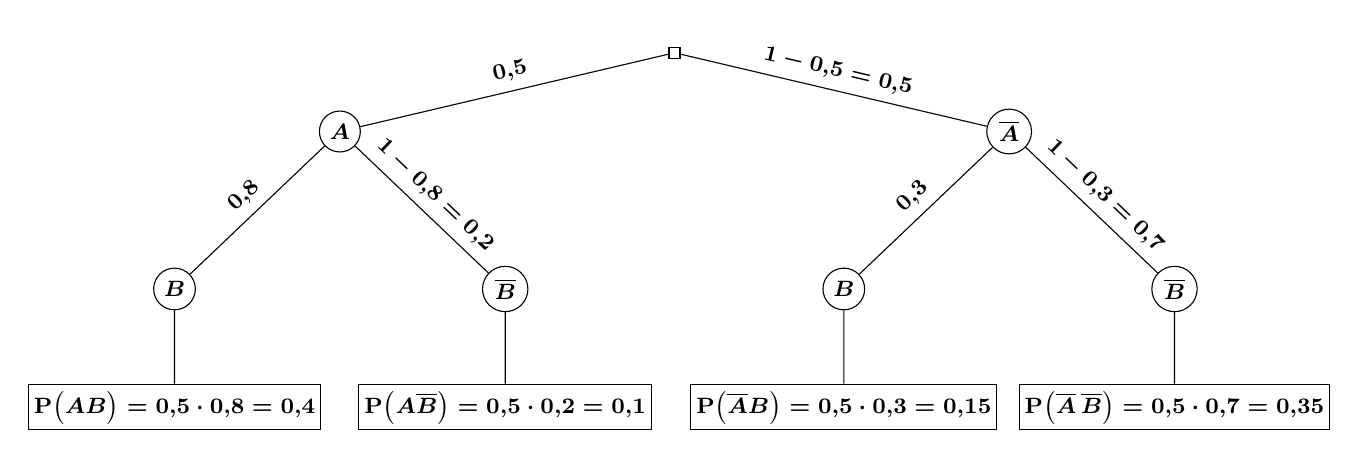
\begin{tikzpicture}[font=\footnotesize]
					\mathversion{bold} 
					 \tikzset{
						level 1/.style={level  distance=10mm,sibling distance=85mm},
						level 2/.style={level distance=20mm,sibling distance=42mm}, 
						level 3/.style={level distance=15mm,sibling distance=40mm}, 
						level  4/.style={level distance=15mm,sibling distance=50mm},
						solid node/.style={circle,draw,inner  sep=2},
						hollow node/.style={rectangle,draw,inner  sep=2},
					 }
					 \node[hollow node,label=above:{}]{}
						 child{node[solid node]{$A$}
						child{node (l1)[solid  node] {$B$}
						child{node[hollow node] {$\mathbf{P}\big (AB\big)=0{,}5 \cdot 0{,}8=0{,}4$}  edge from parent node[left]{}}
						edge from parent  node [sloped,midway,above]{$0{,}8$}
					 }
						child{node (l2)[solid  node]{$\overline{B}$}
						child{node[hollow node]{$\mathbf{P}\big (A\overline{B}\big)=0{,}5 \cdot 0{,}2=0{,}1$} edge from parent node[left]{}} 
						edge from  parent node [sloped,midway,above]{$1-0{,}8=0{,}2$}
					 }
						edge from parent node  [sloped,midway,above]{$0{,}5$}
					} 
						 child{node[solid node]{$\overline{A}$}
						child{node  (r1)[solid node]{$B$}
						child{node[hollow node]{$\mathbf{P}\big (\overline{A}B\big)=0{,}5  \cdot 0{,}3=0{,}15$} edge from parent node[left]{}}
						 edge from parent node [sloped,midway,above]{$0{,}3$}
					} 
						child{node (r2)[solid  node]{$\overline{B}$}
						 child{node[hollow node]{$\mathbf{P}\big (\overline{A}\,\overline{B}\big)=0{,}5 \cdot 0{,}7=0{,}35$}edge from parent node[left]{}}
						edge from parent node  [sloped,midway,above]{$1-0{,}3=0{,}7$}
					} 
						edge from parent node [sloped,midway,above]{$1-0{,}5=0{,}5$} 
						}; 
				\end{tikzpicture}
		\end{center}
		\begin{itemchoice}
			\itemch \textbf{Sai}  $\mathrm{P}(B)=\mathrm{P}(AB)+\mathrm{P}(\overline{A}B)=0{,}4+0{,}15=0{,}55$.
			 \itemch \textbf{Sai}
			$\mathrm{P}(B|\overline{A})=0{,}3$. 
			 \itemch \textbf{Đúng}
			Xác suất để ``Cả hai thí nghiệm  thành công'' là $\mathrm{P}(AB)=0{,}4$.
			 \itemch \textbf{Sai}
			Xác suất để thí nghiệm thứ nhất thành công và thí nghiệm  thứ hai không thành công là $\mathrm{P}(A\overline{B})=0{,}1$.
		\end{itemchoice}
	 }
\end{ex}


%%%%%%%%%%%%%%%% TRẢ LỜI NGẮN %%%%%%%%%%%%%%%%

% nguồn: Lop_12_Dai_so_Chuong_6
\begin{bt}%[2D6V1-3]%[ma:3718f79d]
	Điều tra tình hình mắc bệch ung thư phổi của một vùng thấy tỉ lệ người hút thuốc lá và mắc bệnh là $15\%$, tỉ lệ người hút thuốc lá và không mắc bệnh là $25\%$, tỉ  lệ người không hút thuốc lá và không mắc bệnh là $50\%$ và $10\%$ là người không hút thuốc nhưng mắc bệnh. Tỉ lệ mắc bệnh ung thư phổi giữa người hút thuốc lá và không hút thuốc lá là bao nhiêu?
	\shortans{1,5} 
	 \loigiai{
		Gọi biến cố $A$: \lq\lq Người hút thuốc\rq\rq và $B$: \lq\lq Bị  mắc bệnh ung thư phổi\rq\rq.\\
		Theo  đề bài ta có $\mathrm{P} (A\cap B)=0{,}15$; $\mathrm{P} (A\cap \overline{B})=0{,}25$; $\mathrm{P} (\overline{A}\cap \overline{B})=0{,}5$; $\mathrm{P} (\overline{A}\cap B)=0{,}1$.\\
		Suy ra $\mathrm{P} (B)=\mathrm{P}  (A\cap B)+\mathrm{P} (A\cap \overline{B})=0{,}15+0{,}1=0{,}25$.\\
		Xác  suất người đó hút thuốc lá biết họ mắc bệnh ung thư phổi là
		\[\mathrm{P} (A\mid B)=\dfrac{\mathrm{P} (A\cap B)}{\mathrm{P} (B)}=\dfrac{0{,}15}{0{,}25}=0{,}6.\] 
		Xác suất người đó không hút thuốc lá biết  họ mắc bệnh ung thư phổi là
		\[\mathrm{P} (\overline{A}\mid B)=\dfrac{\mathrm{P}  (\overline{A}\cap B)}{\mathrm{P} (B)}=\dfrac{0{,}1}{0{,}25}=0{,}4.\]
		 Vậy tỉ lệ mắc bệnh ung thư phổi giữa người hút thuốc lá và người không hút thuốc lá là $\dfrac{0{,}6}{0{,}4}=1{,}5$.
	} 
\end{bt}

% nguồn: Lop_12_Dai_so_Chuong_6
\begin{bt}%[2D6V1-3]%[ma:eff51912]
	Dây chuyền lắp ráp nhận được các chi tiết máy sản xuất. Trung bình máy  thứ nhất cung cấp $60\%$ chi tiết, máy thứ hai cung cấp $40\%$ chi tiết. Khoảng $90\%$ chi tiết do máy thứ nhất sản suất là đạt tiêu chuẩn, còn $85\%$ chi tiết do máy thứ hai sản suất là đạt tiêu chuẩn. Lấy ngẫu nhiên từ dây chuyền một sản phẩm, thấy nó đạt chuẩn. Tìm xác suất để sản phẩm đó do máy thứ nhất sản xuất (làm tròn đến hàng phần trăm).
	\shortans{0,61} 
	\loigiai{ 
		Gọi $A$ là biến cố:  \lq\lq Chọn được sản phẩm từ máy thứ nhất\rq\rq.\\
		Gọi $B$  là biến cố: \lq\lq Chọn được sản phẩm đạt chuẩn\rq\rq.\\
		Ta lập  sơ đồ hình cây như hình bên dưới.\\
		\begin{center}
			\begin{tikzpicture}[declare function={dai=3; cao=0.65;},>=stealth,font = \footnotesize,line join=round,line cap=round,>=stealth,scale=1]
					 \tikzset{nhan/.style={draw,circle,minimum size=30pt,font = \footnotesize,inner sep=0pt}}
					\path (0,0) node[nhan] (G){Dây chuyền} 
						(dai,{1.5*cao}) node[nhan] (B) {$A$} 
						(dai,{-1.5*cao}) node[nhan] (nB)  {$\overline{A}$}
						({2*dai},{3*cao}) node[nhan] (BA) {$B$} 
						 ({2*dai},{cao}) node[nhan] (BnA) {$\overline{B}$}
						({2*dai},{-cao}) node[nhan]  (nBA) {$B$}
						({2*dai},{-3*cao}) node[nhan] (nBnA) {$\overline{B}$}; 
					\draw[->]  (G.0)--(B.200) node[sloped,pos=0.5,above]{$0{,}6$};
					 \draw[->] (G.0)--(nB.160) node[sloped,pos=0.5,below]{$0{,}4$};
					 \draw[->] (B.10)--(BA.190) node[sloped,pos=0.5,above]{$0{,}9$};
					 \draw[->] (B.10)--(BnA.170) node[sloped,pos=0.5,below]{$0{,}1$};
					 \draw[->] (nB.-10)--(nBA.190) node[sloped,pos=0.5,above]{$0{,}85$};
					\draw[->]  (nB.-10)--(nBnA.170) node[sloped,pos=0.5,below]{$0{,}15$};
					 \node at (0,0){\href{2XCB1D}{\tiny \phantom{2XCB1D}}};
				\end{tikzpicture}
		\end{center}
		Xác suất sản phẩm được chọn đạt chuẩn do máy  thứ nhất sản xuất là
		\[\mathrm{P} (C\mid B)=\dfrac{\mathrm{P} (A\cap B)}{\mathrm{P}  (B)}=\dfrac{0{,}6\cdot0{,}9}{0{,}6\cdot0{,}9+0{,}4\cdot0{,}85}=\dfrac{27}{44}\approx 0{,}61.\]
	} 
\end{bt}

% nguồn: Lop_12_Dai_so_Chuong_6
\begin{bt}%[2D6C1-3]%[ma:52e8dbca]
	Một thành phố có ba loại phương tiện giao thông công cộng: xe buýt, tàu điện ngầm và taxi. Tỉ lệ sử dụng mỗi loại phương tiện đối với xe buýt $40\%$, tàu điện ngầm $35\%$, taxi $25\%$. Tỉ lệ trễ giờ của xe buýt, tàu  điện ngầm và taxi trong một tháng lần lượt là: $20\%$,\,$10\%$,\,$5\%$. Anh Lộc là một người dân trong thành phố. Trong tháng đầu tiên, anh Lộc chọn một trong ba loại phương tiện trên để đi làm, sao cho xác suất chọn mỗi loại phương tiện đúng bằng tỉ lệ sử dụng phương tiện đó của người dân trong thành phố. Từ tháng thứ hai trở đi, cách anh Lộc chọn phương tiện đi làm phụ thuộc vào việc anh có bị trễ giờ trong tháng trước hay không: Nếu tháng trước anh Lộc không bị trễ giờ thì anh ấy tiếp tục sử dụng loại phương tiện mà anh đã đi trong tháng đó; Nếu tháng trước anh Lộc bị trễ giờ thì anh ấy sẽ chọn ngẫu nhiên một trong hai loại phương tiện còn lại để đi làm trong tháng tiếp theo, với xác suất chọn mỗi loại phương tiện là $50\%$. Xác suất để anh Lộc sử dụng taxi trong tháng thứ ba có bằng $\dfrac{a}{b}$, (với $\dfrac{a}{b}$ là phân số tối giản). Tính $b-2a$.
	 \shortans{5354}
	 \loigiai{
		 Gọi $A_i,\,B_i,\,\mathrm{C}_i$ lần lượt là các biến cố: \lq\lq Anh Lộc chọn phương tiện là xe buýt, tàu điện ngầm và taxi ở tháng thứ $i$ ( $i=1;2;3;\ldots$)\rq\rq.\\
		Gọi $T$ là biến cố: \lq\lq Anh Lộc  bị trễ\rq\rq.\\
		Ta có $\mathrm{P} ( {T}\mid{A_i}\;)=0{,}2$; $\mathrm{P} ( {T}\mid{B_i}\;)=0,1$;  $\mathrm{P} ( {T}\mid{\mathrm{C}_i}\;)=0{,}05$.\\
		 Đặt $\mathrm{P} ( A_i)=x_i$; $\mathrm{P} ( B_i)=y_i$; $\mathrm{P} ( \mathrm{C}_i)=z_i$. \\
		Ta có sơ đồ cây như hình vẽ  bên dưới.\\
		\begin{center}
			\begin{tikzpicture}[
						 state/.style={circle,draw,fill=blue!10,inner sep=2pt},
						start/.style={circle,draw,inner  sep=1.5pt},
						prob/.style={midway,fill=white,inner sep=1pt,font=\small,text=blue}] 
					\node[start] (Root) at  (0,0) {};
					\node[state] (Ai) at  (3,6) {$A_i$};
					\node[state] (Bi) at (5,0) {$B_i$}; 
					\node[state] (Ci) at  (3,-6) {$\mathrm{C}_i$};
					\draw (Root) --  node[midway,above,sloped,font=\small] {$x_i$}
						(Ai); 
					\draw (Root)  -- node[midway,above,font=\small] {$y_i$}
						(Bi); 
					\draw (Root) -- node[midway,below,sloped,font=\small] {$z_i$} 
						 (Ci);
					\node[state,above right=1cm of Ai] (T_Ai) {$T$}; 
					\node[state,above  right=2.5cm of T_Ai] (Bi+1_from_T_Ai) {$B_{i+1}$};
					 \node[state,below=1cm of Bi+1_from_T_Ai] (Ci+1_from_T_Ai) {$\mathrm{C}_{i+1}$};
					\node[state,right=2.5cm of Ai,below=2cm of  T_Ai] (Tbar_Ai) {$\overline{T}$};
					\node[state,right=2.5cm of Tbar_Ai]  (Ai+1_from_Tbar_Ai) {$A_{i+1}$};
					\draw (Ai)  -- node[prob,above,sloped] {0,2}
						(T_Ai); 
					\draw (Ai) -- node[prob,below,sloped]  {0,8}
						(Tbar_Ai); 
					\draw (T_Ai) --  node[prob,above,sloped] {0,5}
						 (Bi+1_from_T_Ai);
					 \draw (T_Ai) -- node[prob,below,sloped] {0,5}
						(Ci+1_from_T_Ai); 
					\draw  (Tbar_Ai) -- node[prob,above] {1}
						 (Ai+1_from_Tbar_Ai);
					 \node[state,right=2cm of Bi,above right=2cm] (T_Bi) {$T$};
					 \node[state,above right=1.5cm of T_Bi] (Ai+1_from_T_Bi) {$A_{i+1}$};
					 \node[state,below=1cm of Ai+1_from_T_Bi] (Ci+1_from_T_Bi) {$\mathrm{C}_{i+1}$};
					\node[state,right=2cm of Bi,below right=1.5cm] (Tbar_Bi) {$\overline{T}$}; 
					 \node[state,right=1.5cm of Tbar_Bi] (Bi+1_from_Tbar_Bi) {$B_{i+1}$};
					\draw  (Bi) -- node[prob,above,sloped] {0,1}
						(T_Bi); 
					\draw (Bi) --  node[prob,below,sloped] {0,9}
						 (Tbar_Bi);
					\draw (T_Bi) --  node[prob,above,sloped] {0,5}
						(Ai+1_from_T_Bi); 
					\draw (T_Bi) -- node[prob,below,sloped] {0,5} 
						 (Ci+1_from_T_Bi);
					\draw (Tbar_Bi)  -- node[prob,above] {1}
						 (Bi+1_from_Tbar_Bi);
					\node[state,right=2.5cm of Ci,above  right=2cm] (T_Ci) {$T$};
					\node[state,above right=1.5cm of T_Ci] (Ai+1_from_T_Ci) {$A_{i+1}$}; 
					\node[state,below=1.5cm of Ai+1_from_T_Ci] (Bi+1_from_T_Ci)  {$B_{i+1}$};
					\node[state,right=2.5cm of Ci,below  right=1.5cm] (Tbar_Ci) {$\overline{T}$};
					\node[state,right=2.5cm of Tbar_Ci] (Ci+1_from_Tbar_Ci)  {$\mathrm{C}_{i+1}$};
					\draw (Ci) --  node[prob,above,sloped] {0,05}
						 (T_Ci);
					 \draw (Ci) -- node[prob,below,sloped] {0,95}
						 (Tbar_Ci);
					\draw (T_Ci) -- node[prob,above,sloped] {0,5} 
						(Ai+1_from_T_Ci); 
					 \draw (T_Ci) -- node[prob,below,sloped] {0,5}
						 (Bi+1_from_T_Ci);
					\draw  (Tbar_Ci) -- node[prob,above] {1}
						 (Ci+1_from_Tbar_Ci);
				\end{tikzpicture}
		\end{center}
		Từ sơ  đồ cây ta có\\
		$\mathrm{P} ( {A_{i+1}})=1\cdot 0{,}8\cdot x_i+0{,}5\cdot 0{,}1\cdot  y_i+0{,}5\cdot 0{,}05\cdot z_i$.\\
		 $\mathrm{P} ( {B_{i+1}})=0{,}5\cdot 0{,}2\cdot x_i+1\cdot0{,}9\cdot y_i+0{,}5\cdot 0{,}05\cdot z_i$.\\
		$\mathrm{P} ( {\mathrm{C}_{i+1}})=0{,}5\cdot 0{,}2\cdot x_i+0{,}5\cdot0{,}1\cdot y_i+1\cdot 0{,}95\cdot z_i$.\\ 
		Mà $x_1=0{,}4$;  $y_1=0{,}35$; $z_1=0{,}295$.\\
		Vậy  $z_1=\dfrac{5\,323}{16\,000}\Rightarrow a=5\,323,\,b=16\,000\Rightarrow b-2a=5\,354$.
	} 
\end{bt}
